% \chapter{Related Works}
\chapter{SRAM PUF Applications}

\section{Key Generator}

In this section, there are two scheme for key generation produced by Hyunho Kang et. al. Both constructions were built on 2014. The first construction, shown in \ref{fig:cryptographic_key_generation_old}, is utilizing random number generator (RNG). This design was perfected in the second design shown in \ref{fig:cryptographic_key_generation}. In the second design, random number generator was removed without affecting the security.

\begin{figure}[tph!]
	\centerline{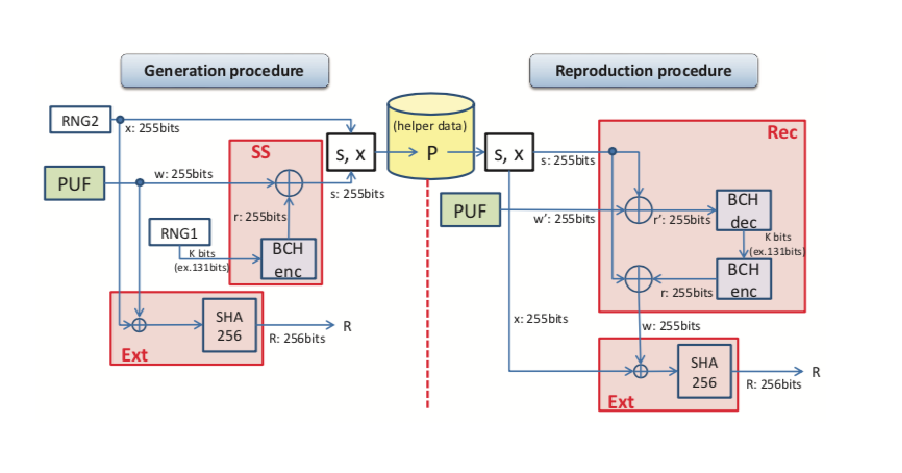
\includegraphics[width={0.5\textwidth}]{images/crypt_key_generation_old}}
% \centerline{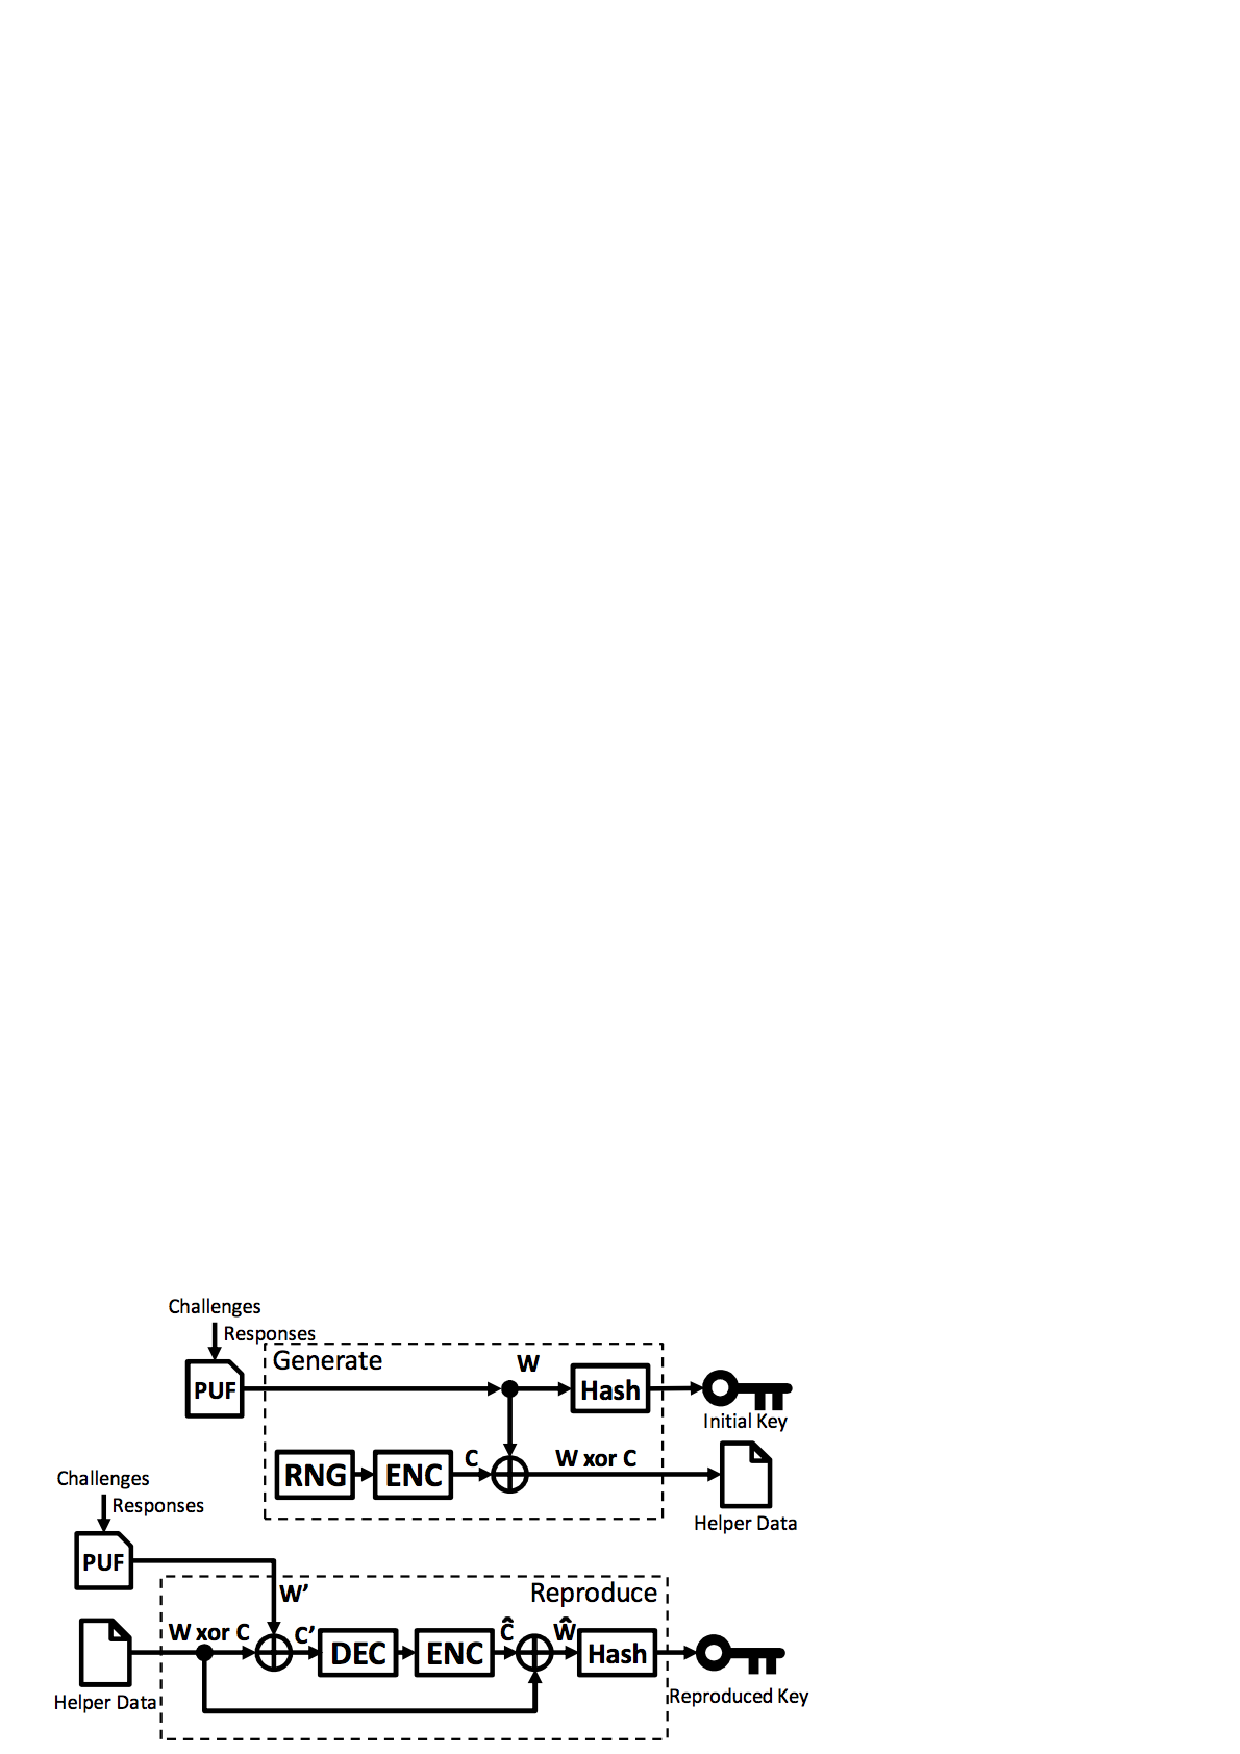
\includegraphics[totalheight=6cm]{images/scheme_stable_key_generation.png}}
    \caption{Implementation diagram using fuzzy extractor (N = 255) \cite{cryptographic_key_generation_old}}
    \label{fig:cryptographic_key_generation_old}
\end{figure}

\begin{figure}[tph!]
	\centerline{\includegraphics[width={0.5\textwidth}]{images/crypt_key_generation}}
% \centerline{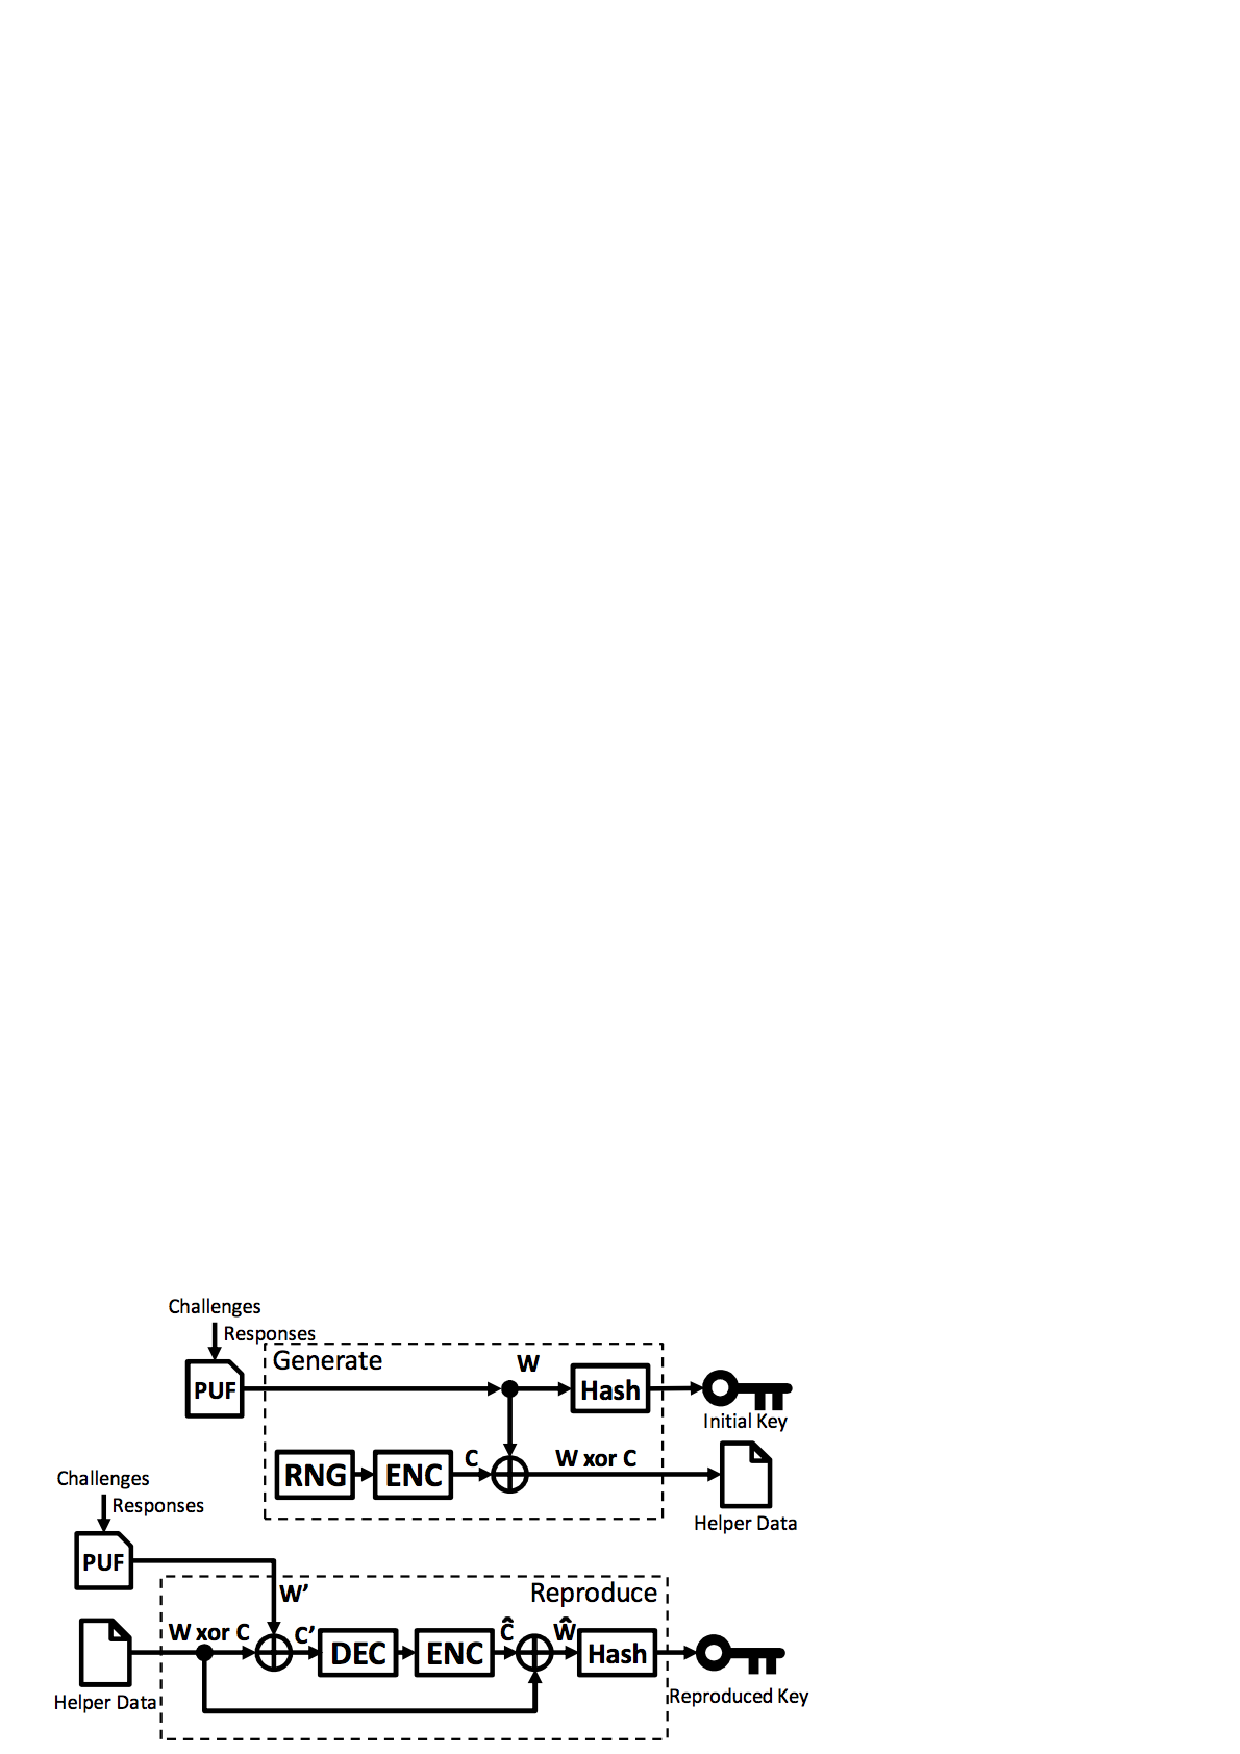
\includegraphics[totalheight=6cm]{images/scheme_stable_key_generation.png}}
    \caption{Implementation diagram for efficient fuzzy extractor based on the syndrome (N = 255) \cite{cryptographic_key_generation}}
    \label{fig:cryptographic_key_generation}
\end{figure}

% \begin{figure}[tph!]
% 	\centerline{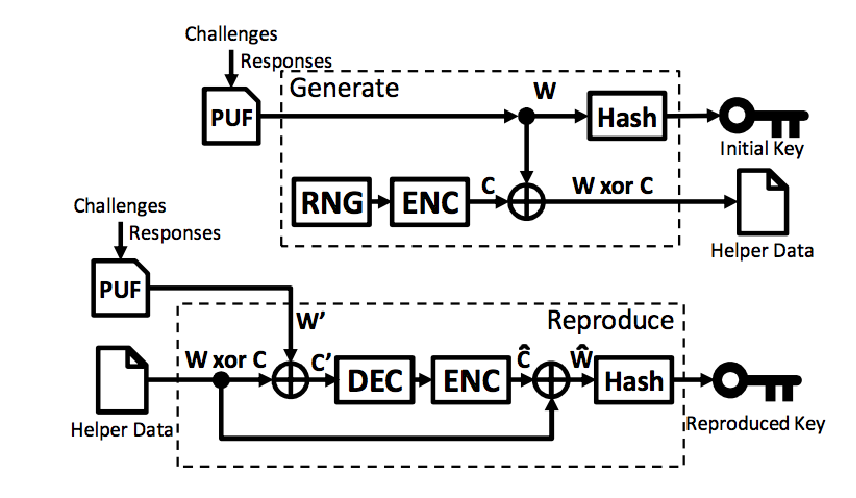
\includegraphics[width={0.5\textwidth}]{images/scheme_stable_key_generation}}
% % \centerline{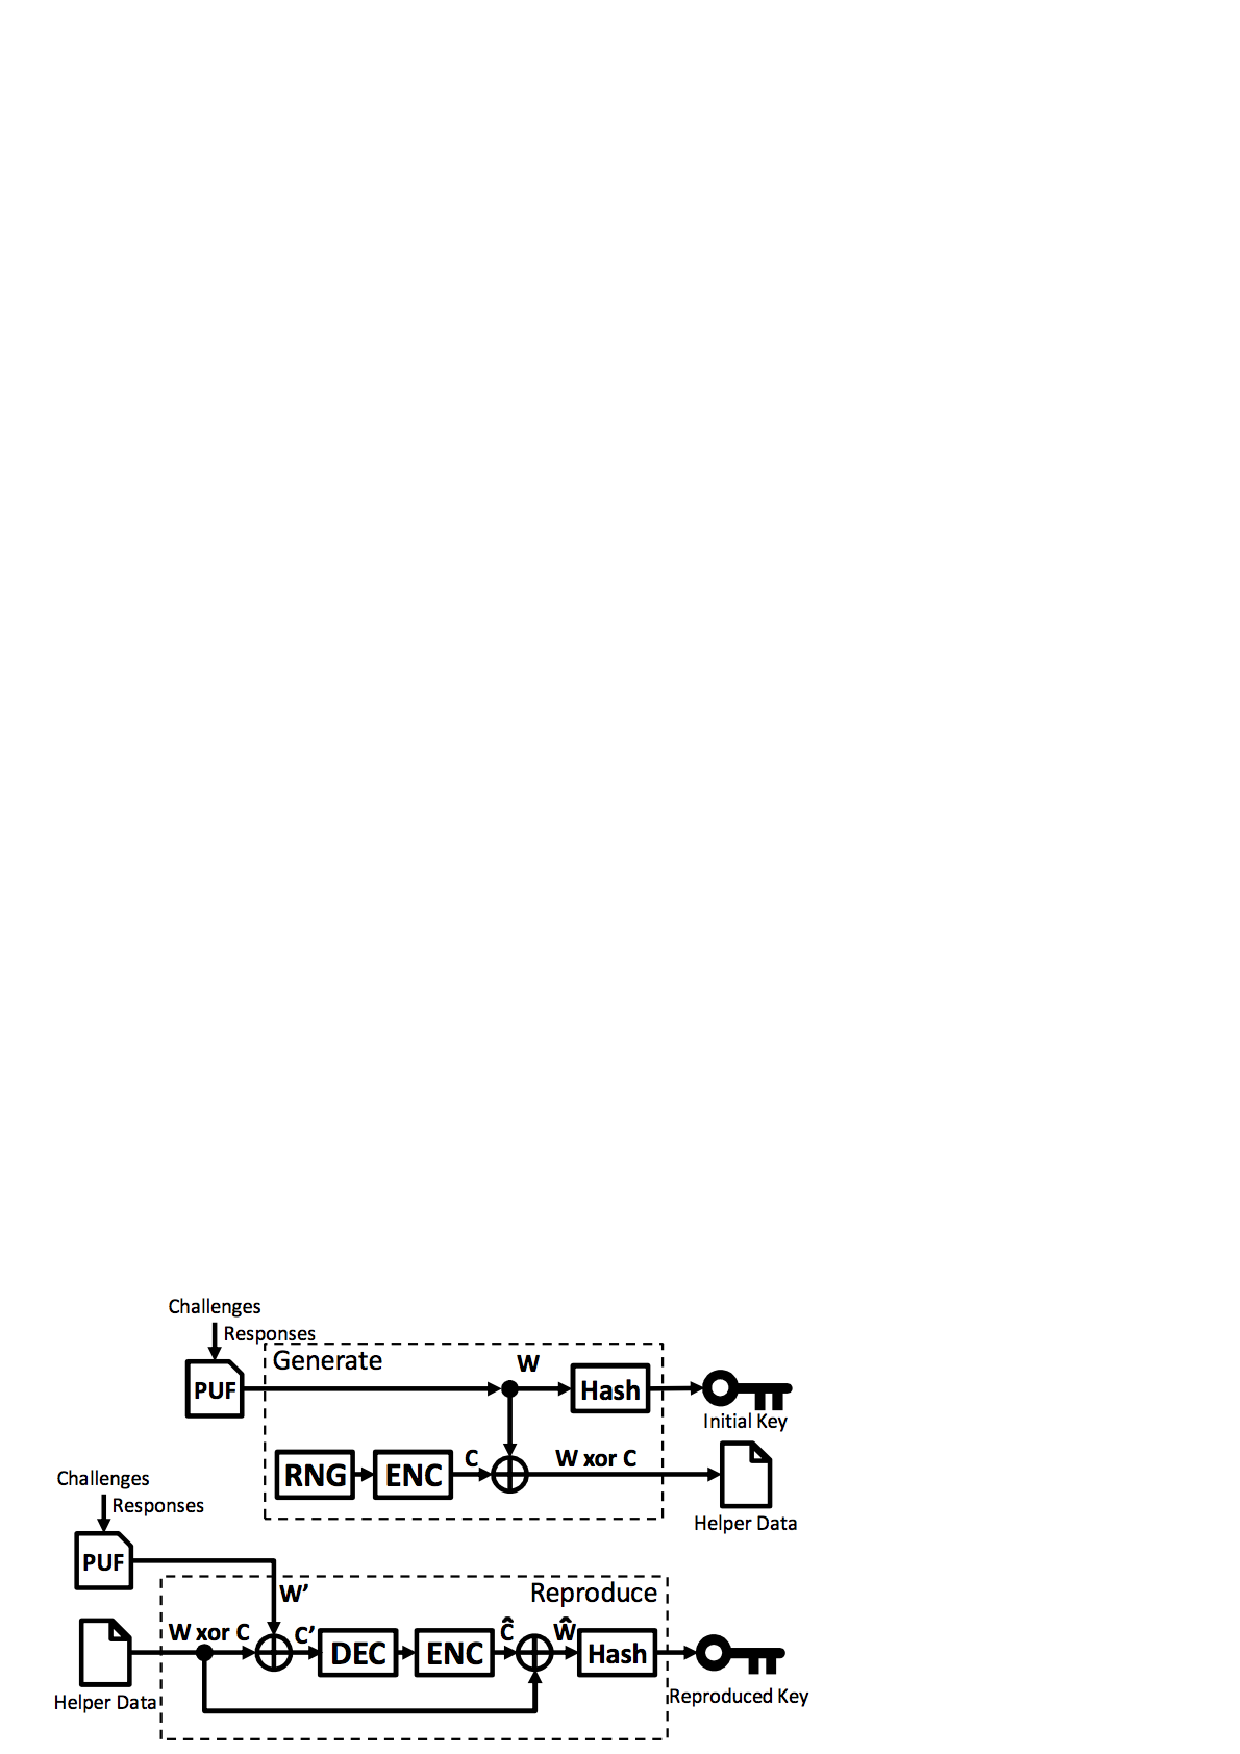
\includegraphics[totalheight=6cm]{images/scheme_stable_key_generation.png}}
%     \caption{Scheme of Stable Key Generation}
%     \label{fig:scheme-key-generator}
% \end{figure}


\section{Key Storage using PUF Scheme}

In a basic key storage scheme using PUF, it usually divided into two phases.  In the first phase, generally called enrollment, the helper data is constructed by XOR-ing PUF bits and the encoded key. In the second phase, which called reconstruction, the helper data is XOR-ed with the PUF bits, followed by decoding the result to reconstruct the key.

% \begin{figure}[tph!]
% \centerline{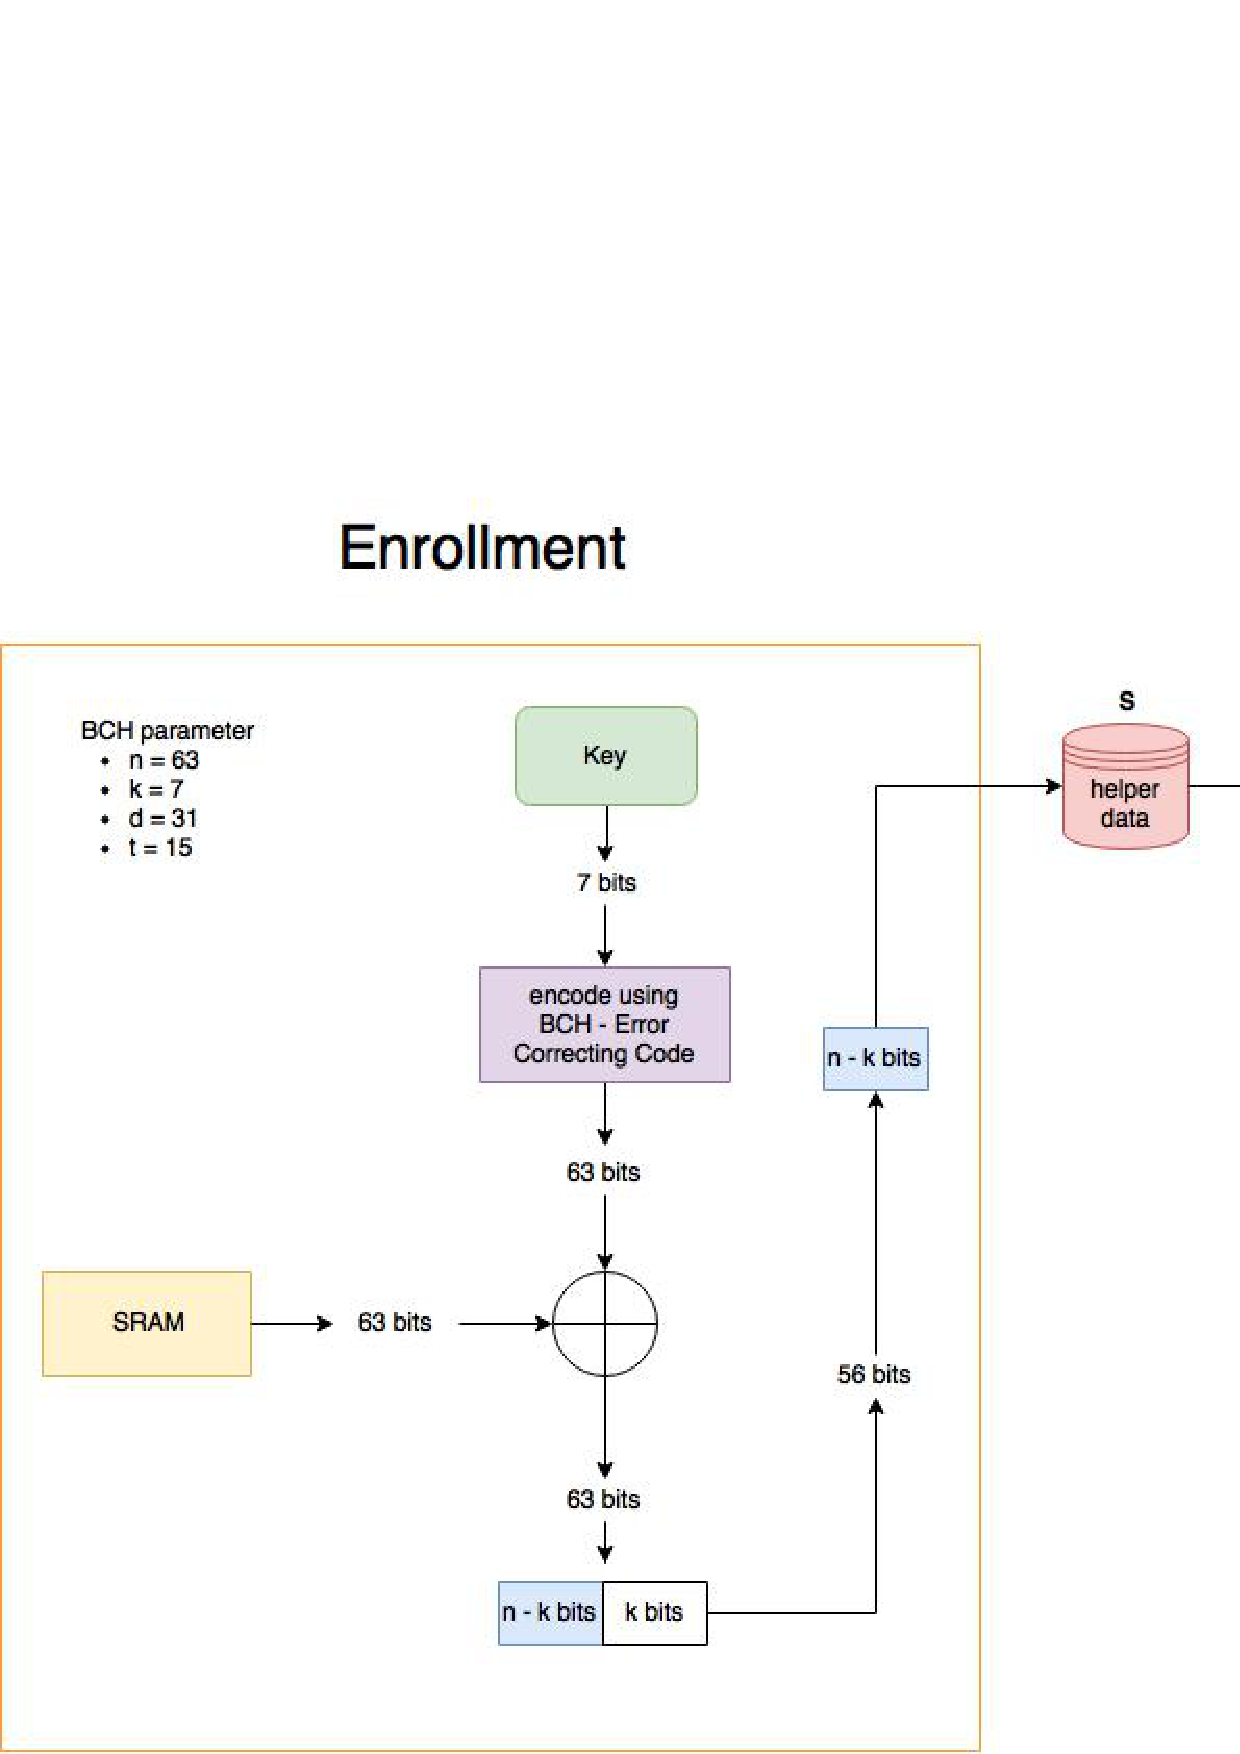
\includegraphics[totalheight=6cm]{images/key-storage-scheme.jpg}}
%     \caption{Scheme for Storing Key}
%     \label{fig:key-storage-scheme}
% \end{figure}


\section{Authentication using PUF Scheme}

In a basic authentication scheme using PUF, it usually divided into two phases.  In the first phase, generally called enrollment, CRPs are generated and stored in a CRP database. In the second phase, usually referred to verification, a challenge from the CRP database is applied to the PUF and the response produced by the PUF is compared with the corresponding response from the database.
